\documentclass{article}
\usepackage[T1]{fontenc}
\usepackage{lmodern}
\usepackage{graphicx}
\usepackage{amsmath,amssymb}
\usepackage[a4paper,margin=2cm]{geometry}
\usepackage[absolute,overlay]{textpos}
\setlength{\TPHorizModule}{1mm}
\setlength{\TPVertModule}{1mm}
\usepackage[indonesian]{babel}
\usepackage{hyperref}
\setlength{\emergencystretch}{2em}
% unit: Halaman 29

\begin{document}

% === Halaman 29 (python/native) ===

29

• Di dalam sistem operasi Unix, ROT13 adalah fungsi menggunakan Caesar 

cipher dengan pergeseran k = 13


Sumber gambar: Wikipedia

% deskripsi: gambar native xref 145
\noindent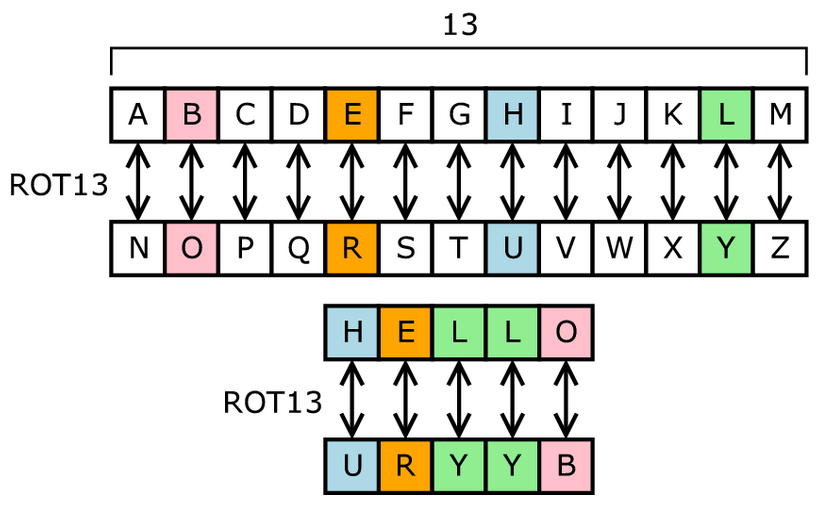
\includegraphics[width=0.85\textwidth]{../../images/python/page_029_img_01.png}

\end{document}
